\documentclass[border=0bp]{standalone}
\usepackage[T1]{fontenc}
\usepackage{newpxtext,newpxmath,graphicx,tikz}
\begin{document}
\begin{tikzpicture}[x=1bp,y=-1bp]
\path[use as bounding box] (0,0) rectangle (859,396);
\node[anchor=north west,inner sep=0pt] at (0,0) {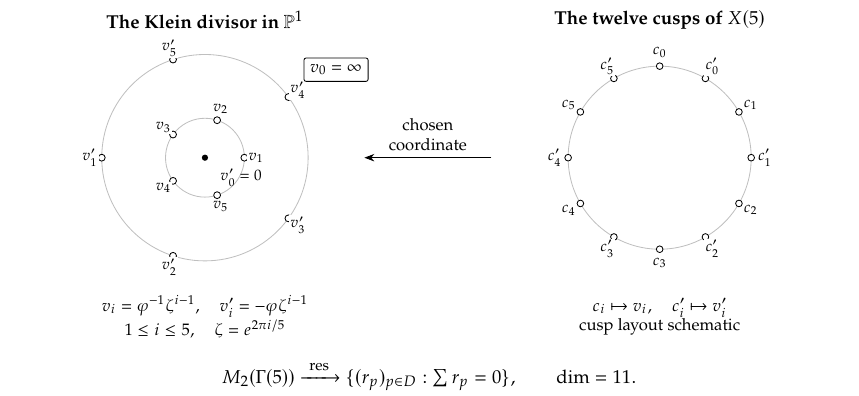
\includegraphics[width=859bp,height=396bp]{fig04_divisor_cusps_original.png}};
\fill[white] (529,319) rectangle (838,349);
\node[anchor=north,inner sep=0pt,text width=309bp,align=center,font=\fontsize{14.5bp}{17bp}\selectfont] at (676,323) {Schematic arrangement of the cusps.};
\end{tikzpicture}
\end{document}
